\documentclass[10pt,a4paper]{article}
\usepackage[utf8x]{inputenc}
\usepackage{ucs}
\usepackage[german]{babel}
\usepackage[left=2.00cm, right=2.00cm, top=2.00cm, bottom=2.00cm]{geometry}
\renewcommand\familydefault{\sfdefault}

\title{Zusammenfassung - Regelungstechnik}
\author{}
\date{2019}

%costum layout
\setlength{\parindent}{0cm}
\usepackage{fancyhdr}
%\usepackage{xcolor}
\pagestyle{fancy}
\fancyhf{}
\fancyhead[L]{
	\strut\rlap{\color{cyan!50!blue}\rule[-\dp\strutbox]{\headwidth}{\headheight}}
	\textcolor {white} {Zusammenfassung: Regelungstechnik}}
\fancyfoot[L]{
	\strut\rlap{\color{cyan!50!blue}\rule[-\dp\strutbox]{\headwidth}{\headheight}}
	\textcolor {white} {zuletzt aktualisiert: \today}}
\fancyhead[R]{\textcolor{white}{Sommersemester 2019}}
%\lfoot{}
\fancyfoot[R]{\textcolor{white} {\thepage}}
%\renewcommand{\footrulewidth}{1pt}

%math
\usepackage{amsmath}
\usepackage{amsfonts}
\usepackage{amssymb}
\usepackage{amstext}
\usepackage{mathtools}

%graphics
\usepackage{graphicx}
\usepackage{floatflt}
\usepackage{float}

%tabular
\usepackage{tabularx}
\usepackage[font=small,labelfont=small]{caption}
\usepackage{colortbl}
\usepackage[dvipsnames]{xcolor}
\renewcommand{\arraystretch}{1.5}
%\arrayrulecolor{white}

%tikz
\usepackage{tikz}
\usetikzlibrary{shapes, petri}
\tikzstyle{ell}=[ellipse,draw, yshift=-2mm]
\tikzstyle{rec} = [rectangle, draw]
\tikzstyle{dia} = [diamond, aspect=2, draw, yshift=-5mm]
\tikzstyle{cir} = [circle, draw, minimum size=3mm]
\tikzstyle{arrHV} = [to path={-| (\tikztotarget)}]
\tikzstyle{arrVH} = [to path={|- (\tikztotarget)}]
\tikzstyle{whileright} = [xshift=20mm, yshift=-3mm]
\tikzstyle{whileleft} = [xshift=-20mm, yshift=-3mm]
\tikzstyle{txtright} = [above, xshift=15mm]
\tikzstyle{txtleft} = [above, xshift=-15mm]
\tikzstyle{empty} = [coordinate]
\usetikzlibrary{positioning}

%listings
\usepackage{listings}
\lstdefinestyle{costum} {
	language=Bash,
	basicstyle=\footnotesize\ttfamily,
	keywordstyle=\bfseries\color{cyan!50!blue},
	commentstyle=\itshape\color{black!50},
	%identifierstyle=\color{blue},
	stringstyle=\color{green!50!black},
	morekeywords={returns, loop, each},
	escapeinside={\%*}{*)}
}
\lstset{style=costum}

%multicol
\usepackage{multicol}
%\setlength{\columnseprule}{0pt}
%\setlength{\columnsep}{20.0pt}



%custom title color
\usepackage{titlesec}
%\titleformat{\section}
%{\color{cyan!80!blue}\normalfont\Large\bfseries}
%{\color{black}\thesection}{1em}{}

%\titleformat{\subsubsection}
%{\color{blue!30!black!70}\normalfont\bfseries}
%{\color{black}\thesection}{1em}{}

\setcounter{secnumdepth}{4}

%\titleformat{\paragraph}
%{\color{green!30!black!70}\normalfont\normalsize\bfseries}{\theparagraph}{1em}{}
%\titlespacing*{\paragraph}
%{0pt}{3.25ex plus 1ex minus .2ex}{1.5ex plus .2ex}

%tab
\newcommand{\tab}[1][1]{\hspace*{#1cm}}

%color_summary
\newcommand{\sumcolor}[1]{\textcolor{red!10!green!40!blue}{#1}}

%coloring
\newcommand{\redr}{\textcolor{red}{r}}
\newcommand{\greeng}{\textcolor{green}{g}}
\newcommand{\blueb}{\textcolor{blue}{b}}

%vector
\newcommand{\vect}[1]{\ensuremath{\begin{bmatrix}#1\end{bmatrix}}}

%other
\usepackage{enumerate}
\usepackage{hyperref}
\usepackage{mathpartir}
\usepackage{trfsigns}
\usepackage{multicol}


%TODO
% Hinweise:
% -----
% Ruhelage
% Partialbruchzerlegung
%
% Fix:
% ---
% 2.1.1 Blockschaltbild P-Glieder



\begin{document}
	\tableofcontents
	\pagebreak
	
\section{Begriff der Regelung}

\subsection{Dynamisches System}
\subsubsection*{Signale und Blöcke:}
\begin{tabularx}{\columnwidth}{llX}
	Bezeichnung & Var. & Beschreibung \\
	\hline
	Ausgangsgröße & $y(t)$ & Ausgangsgröße, der ein gewünschtes Verhalten aufgeprägt werden soll \\
	Stellgröße & $u(t)$ & Eingangsgröße, durch die das System gezielt beeinflusst werden kann \\
	Störgröße & $z(t)$ & Eingangsgröße, die störend und mit zumeist nur ungenau oder gar nicht bekannten Zeitverlauf auf das System wirkt \\
\end{tabularx}

\subsubsection*{Blockschaltbild}
\begin{figure}[H]
	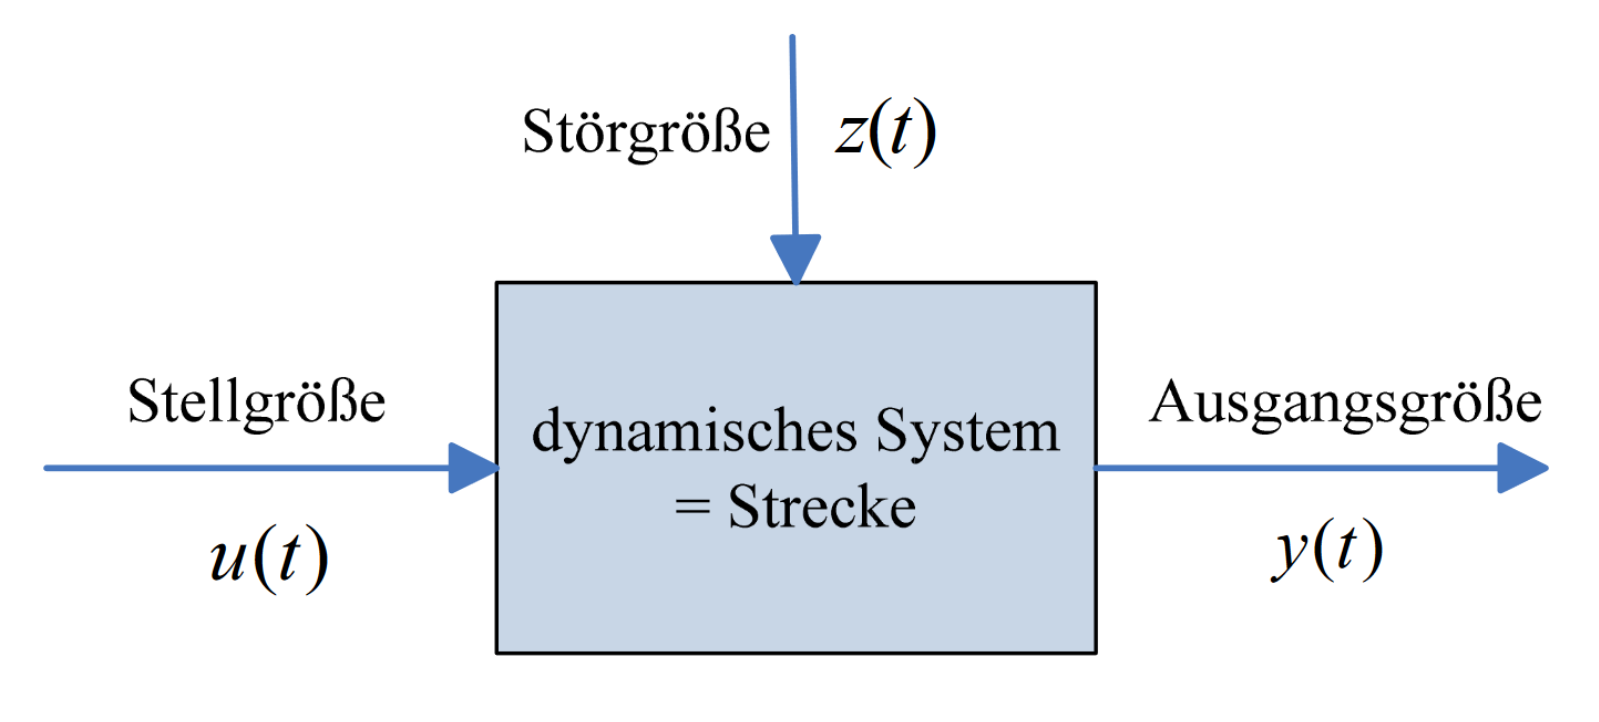
\includegraphics[width=0.5\columnwidth]{imgs/abb1_3.png}
\end{figure}

\subsection{Vorgeschaltete Steuereinrichtung}
\label{steuerung}
\subsubsection*{Ziel}
\begin{itemize}
	\item Übertragungsglied, das den Stellgrößenverlauf $u(t)$ derart generiert, dass $y(t)$ einem vorgegebenen Sollverlauf $w(t)$ folgt.
\end{itemize}

\subsubsection*{Signale und Blöcke:}
\begin{tabularx}{\columnwidth}{llX}
	Bezeichnung & Var. & Beschreibung \\
	\hline
	Führungsgröße & $w(t)$ & Von außen vorgegebener Soll-Verlauf für die Regelgröße y(t) \\
	Ausgangsgröße & $y(t)$ & Ausgangsgröße, der ein gewünschtes Verhalten aufgeprägt werden soll \\
	Stellgröße & $u(t)$ & Eingangsgröße, durch die das System gezielt beeinflusst werden kann \\
	Störgröße & $z(t)$ & Eingangsgröße, die störend und mit zumeist nur ungenau oder gar nicht bekannten Zeitverlauf auf das System wirkt \\
\end{tabularx}

\subsubsection*{Blockschaltbild}
\begin{figure}[H]
	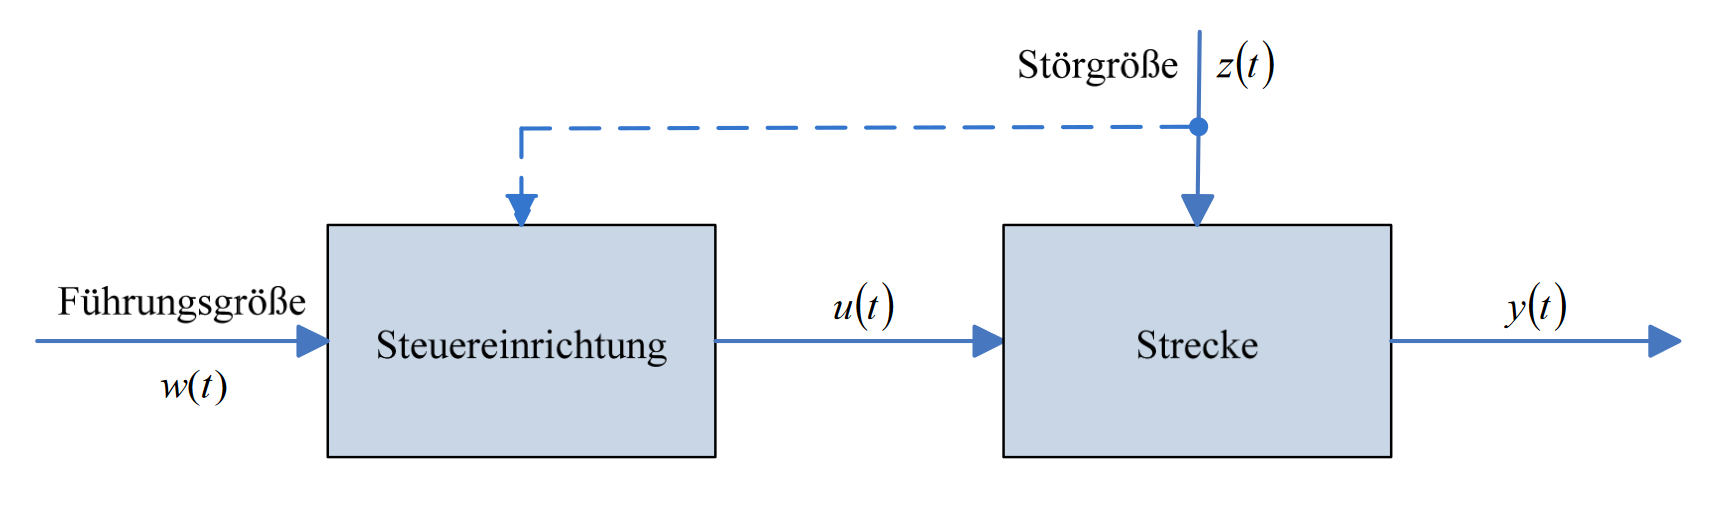
\includegraphics[width=0.8\columnwidth]{imgs/abb1_4.png}
\end{figure}


\subsection{Regelung}
\label{regelung}
\subsubsection*{Ziel:}
\begin{itemize}
		\item Minderung des Einflusses von (nicht-messbaren) Störungen
		\item Minderung des Einflusses von Ungenauigkeiten des Streckenmodells
		\item Verbesserung des Folgeverhaltens
\end{itemize}

\subsubsection*{Signale und Blöcke:}

\begin{tabularx}{\columnwidth}{llX}
	Bezeichnung & Var. & Beschreibung \\
	\hline
	Führungsgröße & $w(t)$ & Von außen vorgegebener Soll-Verlauf für die Regelgröße y(t) \\
	Regelgröße & $y(t)$ & Ausgangsgröße, der ein gewünschtes Verhalten aufgeprägt werden soll \\
	Regelabweichung & $e(t)$ & Entsteht durch Vergleich der Führungsgröße mit der gemessenen Regelgröße und soll klein gehalten werden ($e(t) = w(t) - y'(t)$) \\
	Stellgröße & $u(t)$ & Eingangsgröße, durch die das System gezielt beeinflusst werden kann \\
	Störgröße & $z(t)$ & Eingangsgröße, die störend und mit zumeist nur ungenau oder gar nicht bekannten Zeitverlauf auf das System wirkt \\
	Messrauschen & $n(t)$ & \\
	Regler && Übertragungsglied, das aus der Regelabweichung das Stellsignal $u$ generiert, sodass $y$ möglichst $w$ folgt \\
	Messglied/Messeinrichtung && Erfasst die Regelgröße $y$ mittels eines Sensors und erzeugt ein zu $y(t)$ möglichst äquivalentes Signal $y'(t)$	
\end{tabularx}

\subsubsection*{Blockschaltbild}
\begin{figure}[H]
	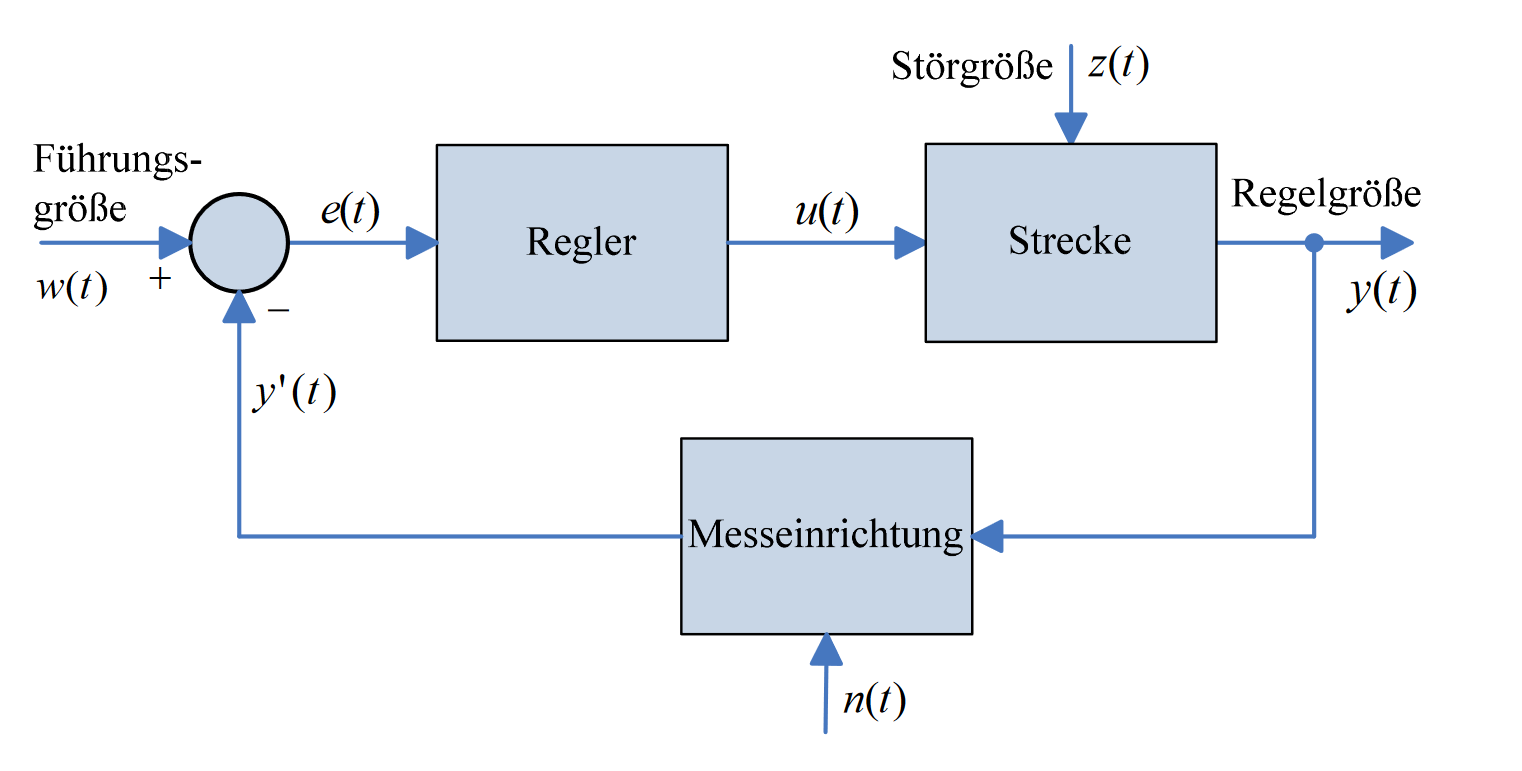
\includegraphics[width=0.8\columnwidth]{imgs/abb1_6.png}
\end{figure}


\subsection{Zwei-Freiheitsgrade-Regelung (Steuerung + Regelung)}
\subsubsection*{Ziel:}
\begin{itemize}
		\item Kombination der Vorteile der Regelschleife (see section \ref{regelung}) und der Vorteile der Steuerung (see section \ref{steuerung})
\end{itemize}

\subsubsection*{Signale und Blöcke:}

\begin{tabularx}{\columnwidth}{llX}
	Bezeichnung & Var. & Beschreibung \\
	\hline
	Führungsgröße & $w(t)$ & Von außen vorgegebener Soll-Verlauf für die Regelgröße y(t) \\
	Regelgröße & $y(t)$ & Ausgangsgröße, der ein gewünschtes Verhalten aufgeprägt werden soll \\
	Regelabweichung & $e(t)$ & Entsteht durch Vergleich der Führungsgröße mit der gemessenen Regelgröße und soll klein gehalten werden ($e(t) = w(t) - y'(t)$) \\
	Stellgröße & $u(t)$ & Eingangsgröße, durch die das System gezielt beeinflusst werden kann \\
	Störgröße & $z(t)$ & Eingangsgröße, die störend und mit zumeist nur ungenau oder gar nicht bekannten Zeitverlauf auf das System wirkt \\
	Regler && Übertragungsglied, das aus der Regelabweichung das Stellsignal $u$ generiert, sodass $y$ möglichst $w$ folgt \\
	Steuereinrichtung && Übertragungsglied, das den Stellgrößenverlauf $u(t)$ derart generiert, dass $y(t)$ einem vorgegebenen Sollverlauf $w(t)$ folgt.
\end{tabularx}

\subsubsection*{Blockschaltbild}
\begin{figure}[H]
	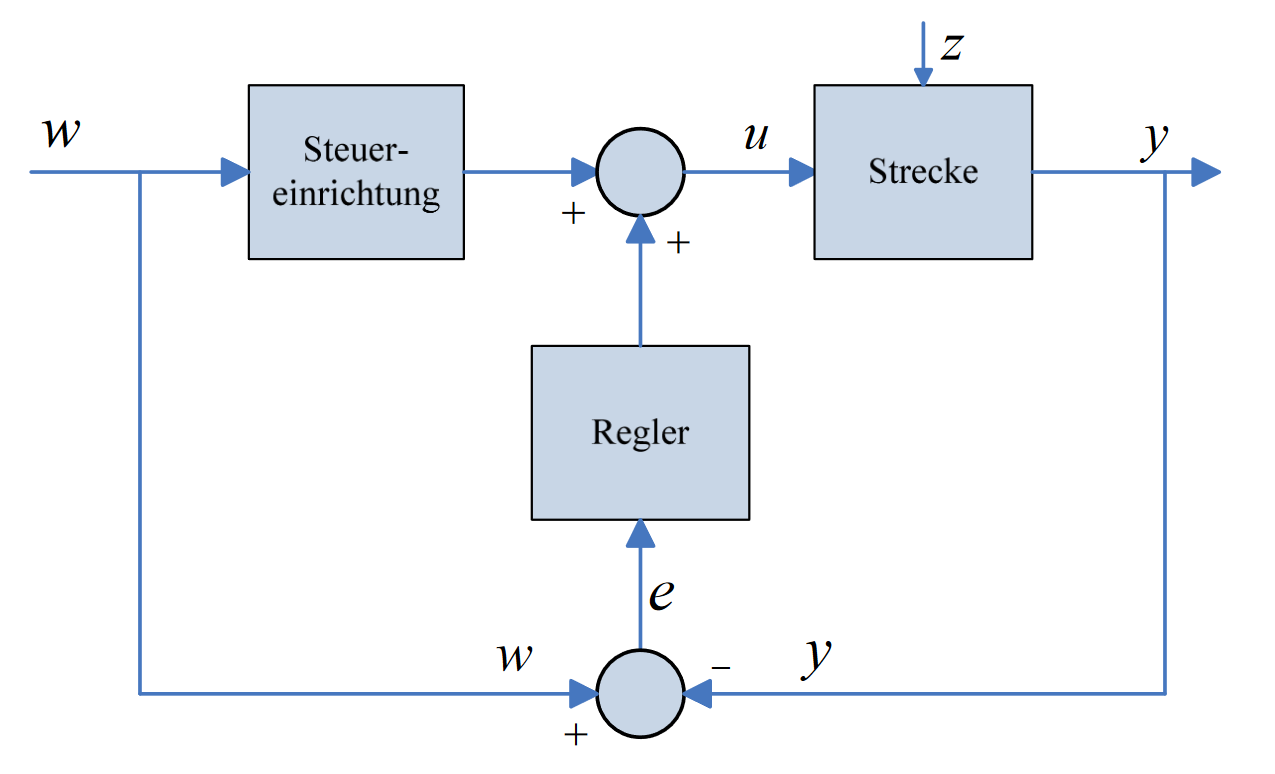
\includegraphics[width=0.8\columnwidth]{imgs/abb1_8.png}
\end{figure}

%TODO evtl Blockschaltbild mit Trajectorienplaner

\subsubsection{Störgrößenaufschaltung}
\subsubsection*{Ziel:}
\begin{itemize}
	\item Mindern des Einflusses einer messbaren Störgröße auf den Ausgang
\end{itemize}

\subsubsection*{Signale und Blöcke:}
\begin{tabularx}{\columnwidth}{llX}
	Bezeichnung & Var. & Beschreibung \\
	\hline
	Führungsgröße & $w(t)$ & Von außen vorgegebener Soll-Verlauf für die Regelgröße y(t) \\
	Regelgröße & $y(t)$ & Ausgangsgröße, der ein gewünschtes Verhalten aufgeprägt werden soll \\
	Regelabweichung & $e(t)$ & Entsteht durch Vergleich der Führungsgröße mit der gemessenen Regelgröße und soll klein gehalten werden ($e(t) = w(t) - y'(t)$) \\
	Stellgröße & $u(t)$ & Eingangsgröße, durch die das System gezielt beeinflusst werden kann \\
	Störgröße & $z_1(t)$ & Messbare Eingangsgröße, die störend auf das System wirkt \\
	Störgröße & $z_2(t)$ & Nicht-Messbare Eingangsgröße, die störend auf das System wirkt \\
	Regler && Übertragungsglied, das aus der Regelabweichung das Stellsignal $u$ generiert, sodass $y$ möglichst $w$ folgt \\
	Steuereinrichtung && Übertragungsglied, das den Stellgrößenverlauf $u(t)$ derart generiert, dass $y(t)$ einem vorgegebenen Sollverlauf $w(t)$ folgt. Besteht aus Störgrößenaufschaltung und Führungsgrößenaufschaltung \\
	Störgrößenaufschaltung && Übertragungspfad zur Aufschaltung einer messbaren Störgröße auf die Stellgröße \\
	Führungsgrößenaufschaltung && Übertragungspfad zur Aufschaltung der Führungsgröße auf die Stellgröße
\end{tabularx}

\subsubsection*{Blockschaltbild}
\begin{figure}[H]
	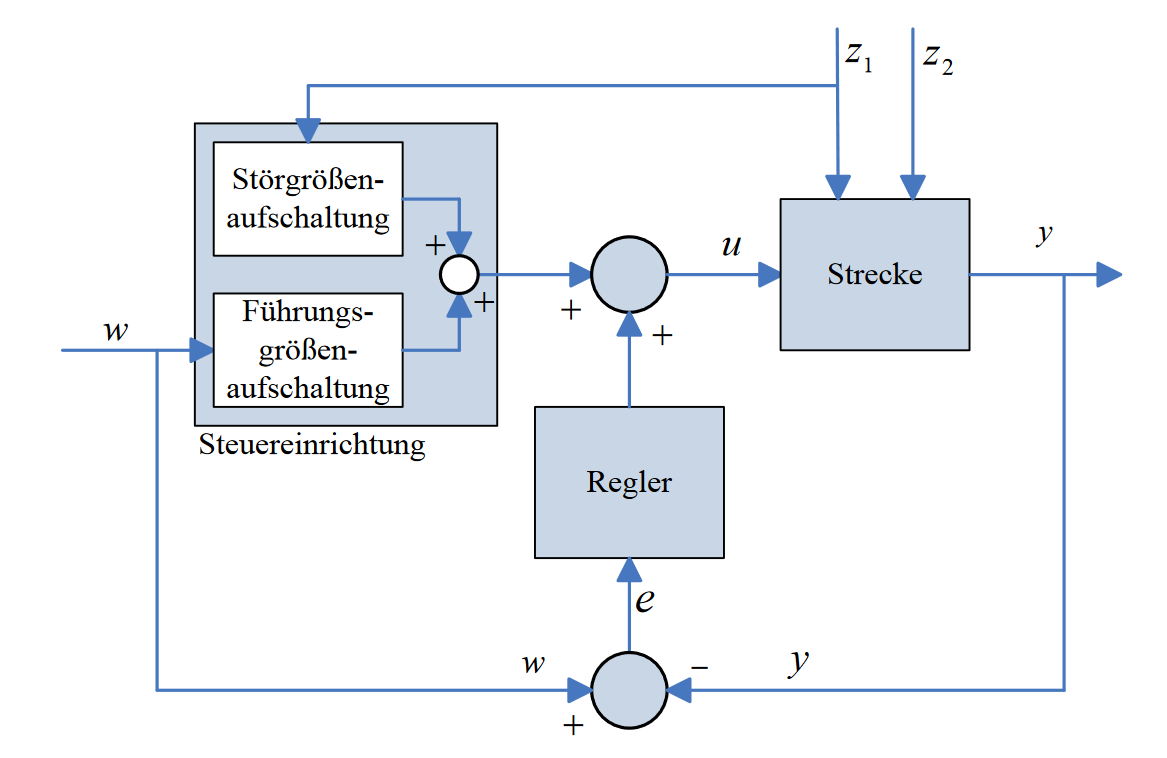
\includegraphics[width=0.8\columnwidth]{imgs/abb1_11.png}
\end{figure}

\section{Modelle}
\subsection{Zustandsdarstellung}
\renewcommand{\arraystretch}{2}
\begin{tabularx}{\columnwidth}{lX}
	Zustandsdarstellung/Zustandsraummodell & Ein Modell bestehend aus
	$$
		\begin{array}{ll}
			\begin{rcases}
				\dot x_1 = f_1(x_1 \dots x_n, z, u) \\
				\tab \vdots \\
				\dot x_n = f_n(x_1 \dots x_n, z, u)
			\end{rcases} & \text{Zustandsdifferentialgleichungen} \\
			y = g(x_1 \dots x_n) & \text{Ausgangsgleichung}
		\end{array}
	$$
	\text{bzw.} 
	$$
		\begin{array}{l}
			\dot{x} = f(x,z,u) \\
			y = g(x)
		\end{array}		
	$$
	wenn bei bekannten Eingangssignalen $u(t)$ und $z(t)$ und gegebenen Anfangswerten $x_1(0), \dots, x_n(0)$ die Zeitverläufe $x_1(t), \dots, x_n(t)$ für $t > 0$ eindeutig bestimmt sind. \\
	Zustandsgleichungen & Zustandsdifferentialgleichungen und die Ausgangsgleichung zusammen \\
	Trajektorie & Die $n$ Zeitverläufe $x_1(t), \dots, x_n(t)$ \\
	Zustandsvariablen & $x_1, \dots, x_n$ \\
	Zustand des Systems & Die Gesamtheit der Werte $x_1, \dots, x_n$ zu einem festen Zeitpunkt $t$ \\
	Zustandsvektor & 
	$$
		x(t) = \vect{x_1(t) \\ \vdots \\ x_n(t)}
	$$	
\end{tabularx}
\renewcommand{\arraystretch}{1.5}

\subsubsection{Zustandsdarstellung bei Linearkombinationen}
Bestehen die rechten Seiten der Zustandsgleichungen ausschließlich aus Linearkombinationen, d.h.:
$$
\begin{array}{l}
	\dot x_1 = a_{11} x_1 + \dots + a_{1n} x_n + e_1 z + b_1 u \\
	\tab \vdots \\
	\dot x_n = a_{n1} x_1 + \dots + a_{nn} x_n + e_n z + b_n u \\
	y = c_1 x_1 + \dots + c_n x_n
\end{array}	
$$
so gilt:
$$
\begin{array}{lcl}
	\dot{x} = A x + e z + b u & ≡ & \vect{\dot x_1 \\ \vdots \\ \dot x_n} = \vect{a_{11} & \dots & a_{1n} \\ \vdots & \ddots & \vdots \\ a_{n1} & \dots & a_{nn}} \vect{x_1 \\ \vdots \\ x_n} + \vect{e_1 \\ \vdots \\ \dot e_n} z(t) + \vect{b_1 \\ \vdots \\ \dot b_n} u(t) \\
	y = c^Tx & ≡ & y = \vect{c_1 & \dots & c_n} \vect{x_1 \\ \vdots \\ x_n}
\end{array}
$$

\paragraph*{Blockschaltbild:} ~\\
\begin{figure}[H]
	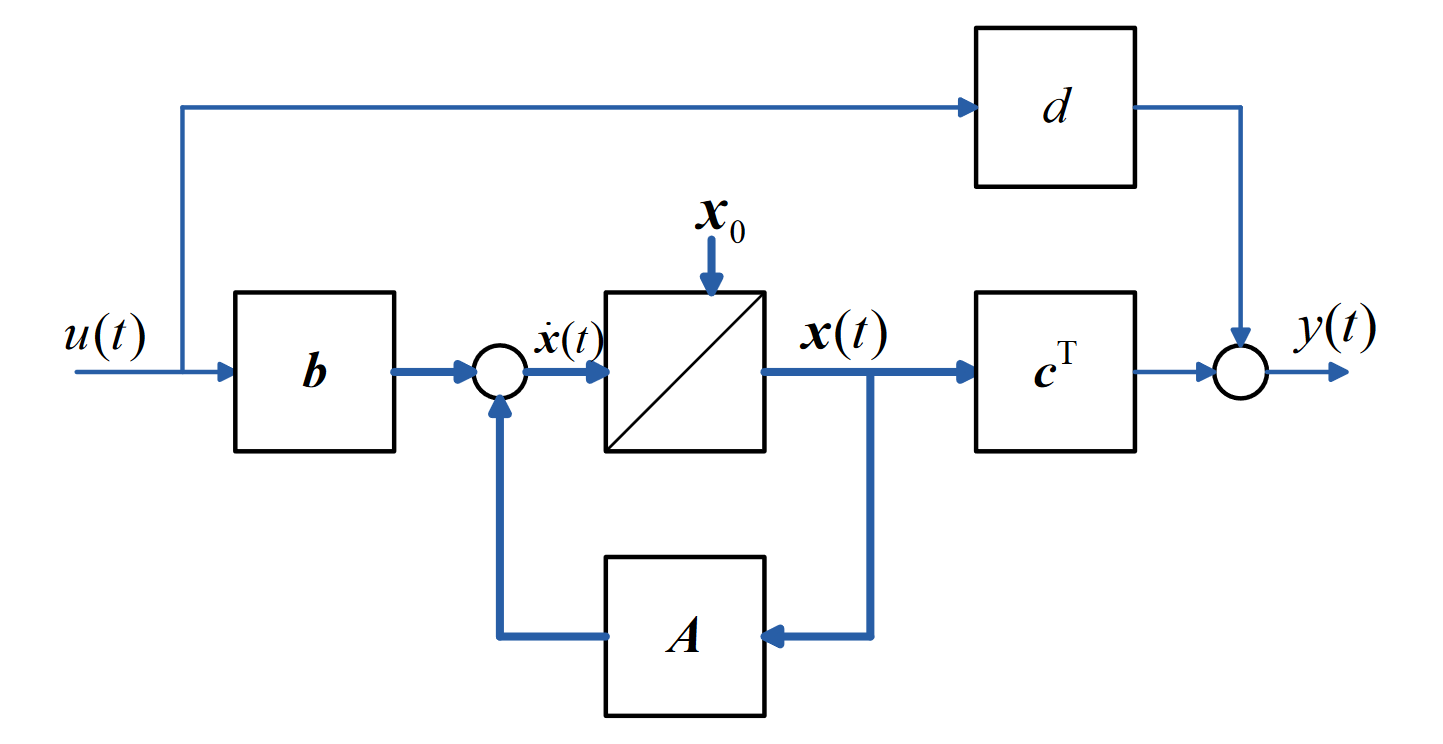
\includegraphics[width=0.8\columnwidth]{imgs/abb2_12.png}
\end{figure}

\subsection{Blockschaltbild}
\subsubsection*{Funktion:}
\begin{itemize}
	\item Das Blockschaltbild ist eine graphische Darstellung der Funktionsbeziehungen zwischen den zeitveränderlichen Größen durch Blöcke und Wirkungslinien. Ein Block ordnet dabei jedem Zeitverlauf der Eingangsgröße eindeutig einen Zeitverlauf der Ausgangsgröße zu und wirkt so als Übertragungsglied.
	Die Zuordnungsvorschrift wird dabei in den Block hineingeschrieben.
\end{itemize}

\subsubsection*{Blockschaltbild:} ~\\
\begin{figure}[H]
	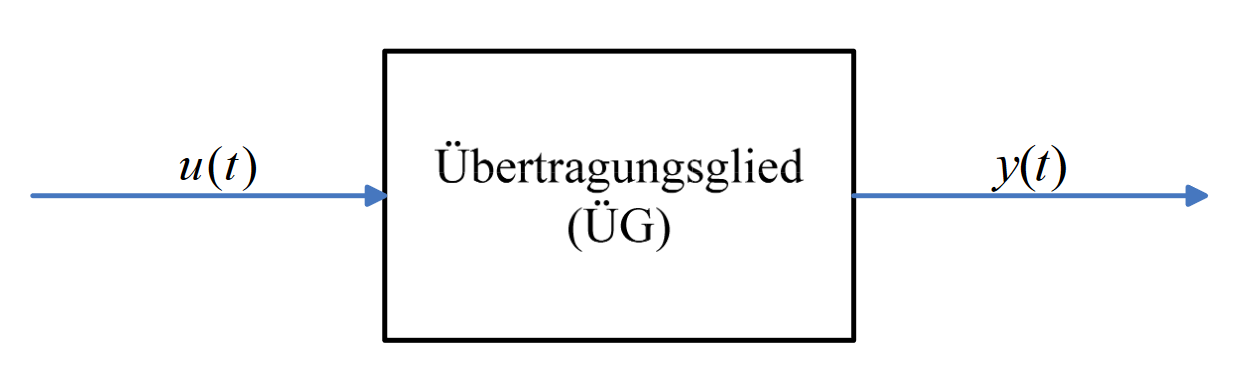
\includegraphics[width=0.8\columnwidth]{imgs/abb2_4.png}
\end{figure}

\subsection{Elementare Übertragungsglieder}
\textbf{Summationsglied:}
\begin{figure}[H]
	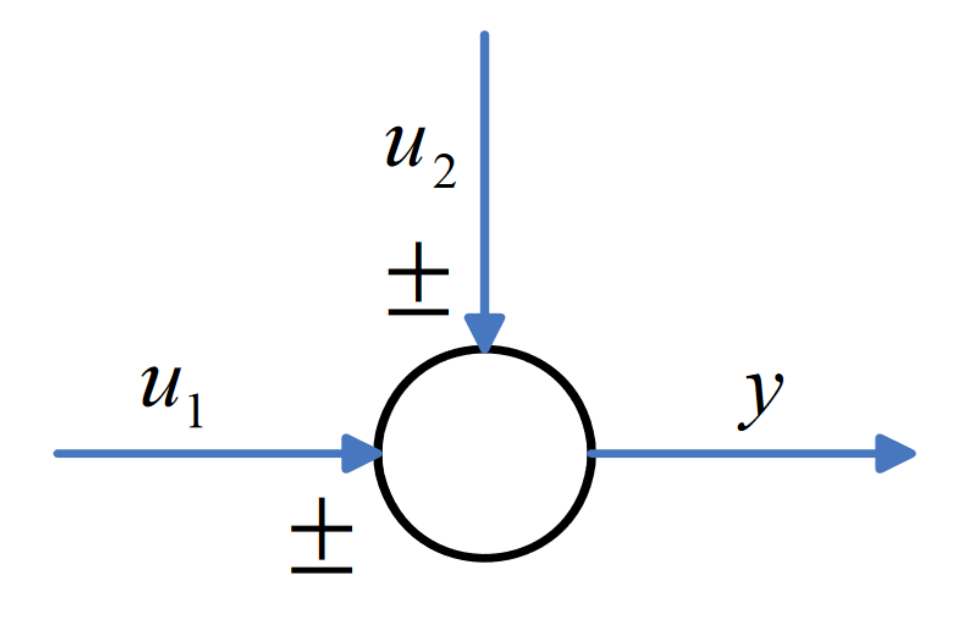
\includegraphics[width=0.2\columnwidth]{imgs/sumglied.png}
\end{figure}

\textbf{Weitere Übertragungsglieder:}
\begin{figure}[H]
	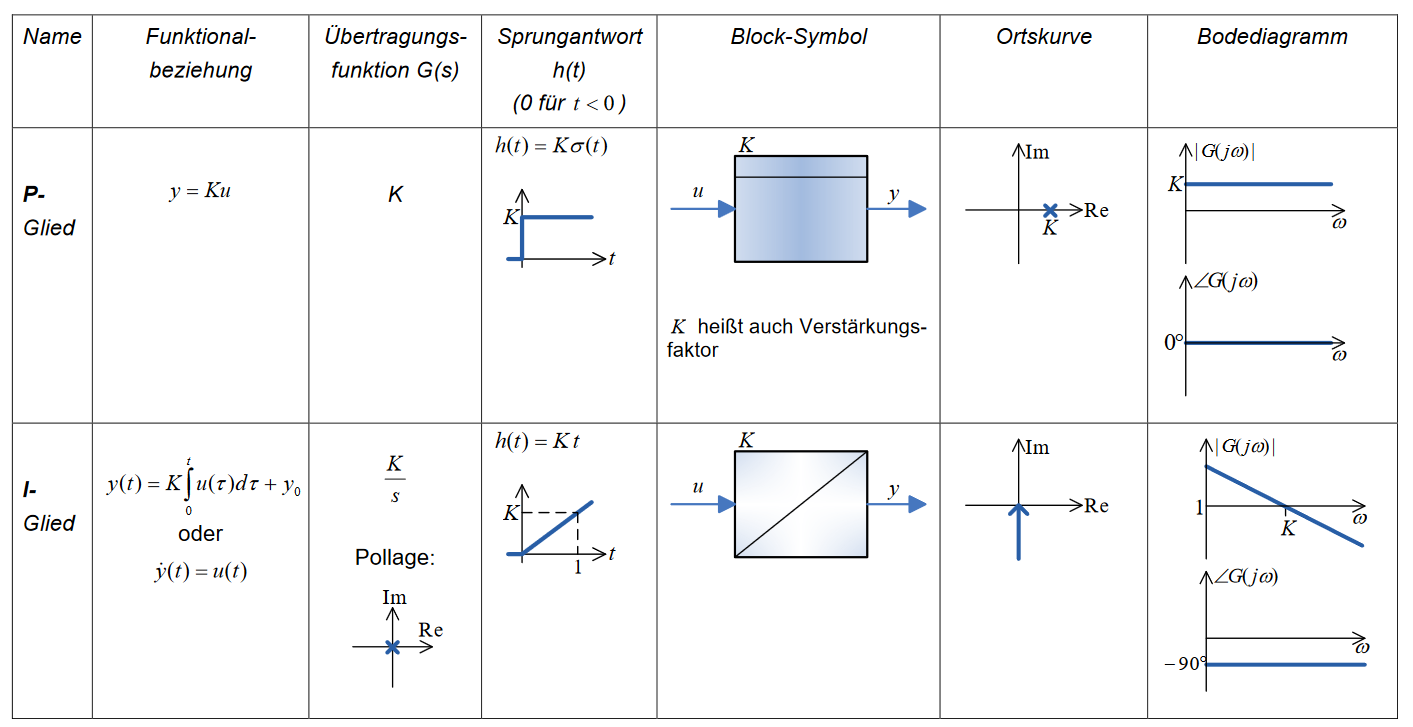
\includegraphics[width=1\columnwidth]{imgs/bb2_2a.png}
\end{figure}
\begin{figure}[H]
	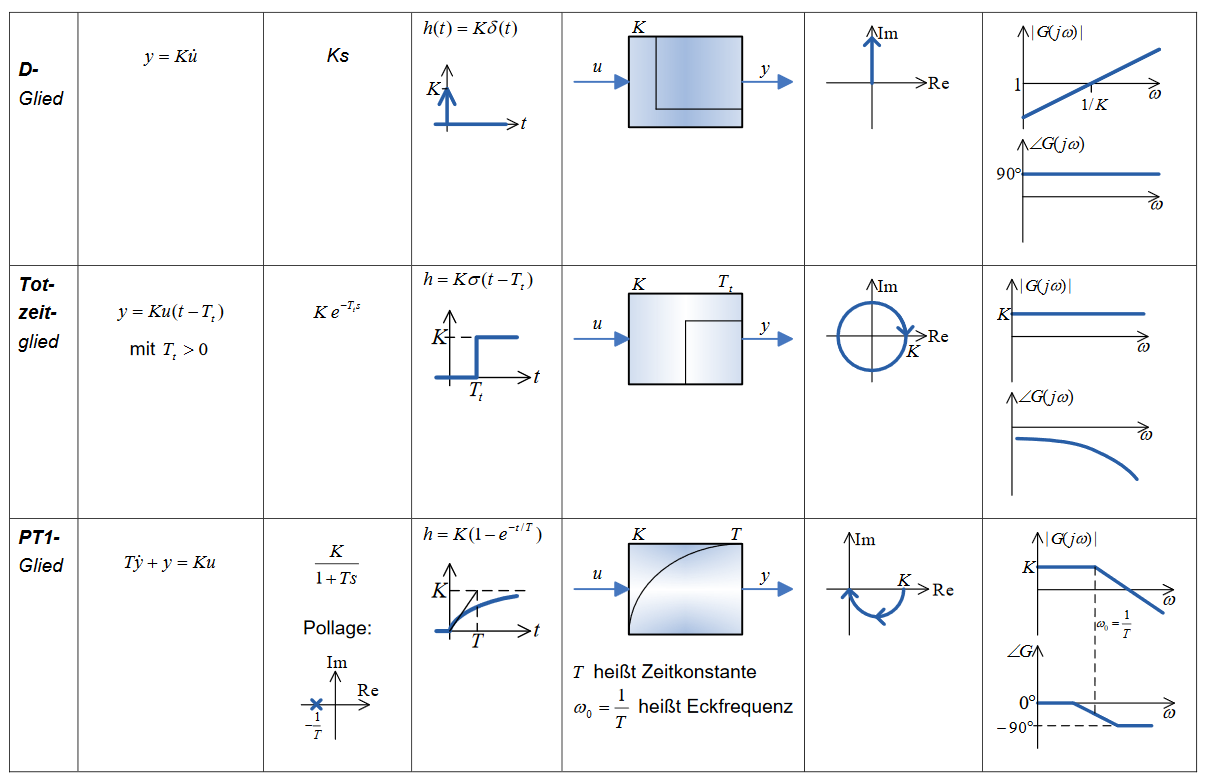
\includegraphics[width=1\columnwidth]{imgs/bb2_2b.png}
\end{figure}
\begin{figure}[H]
	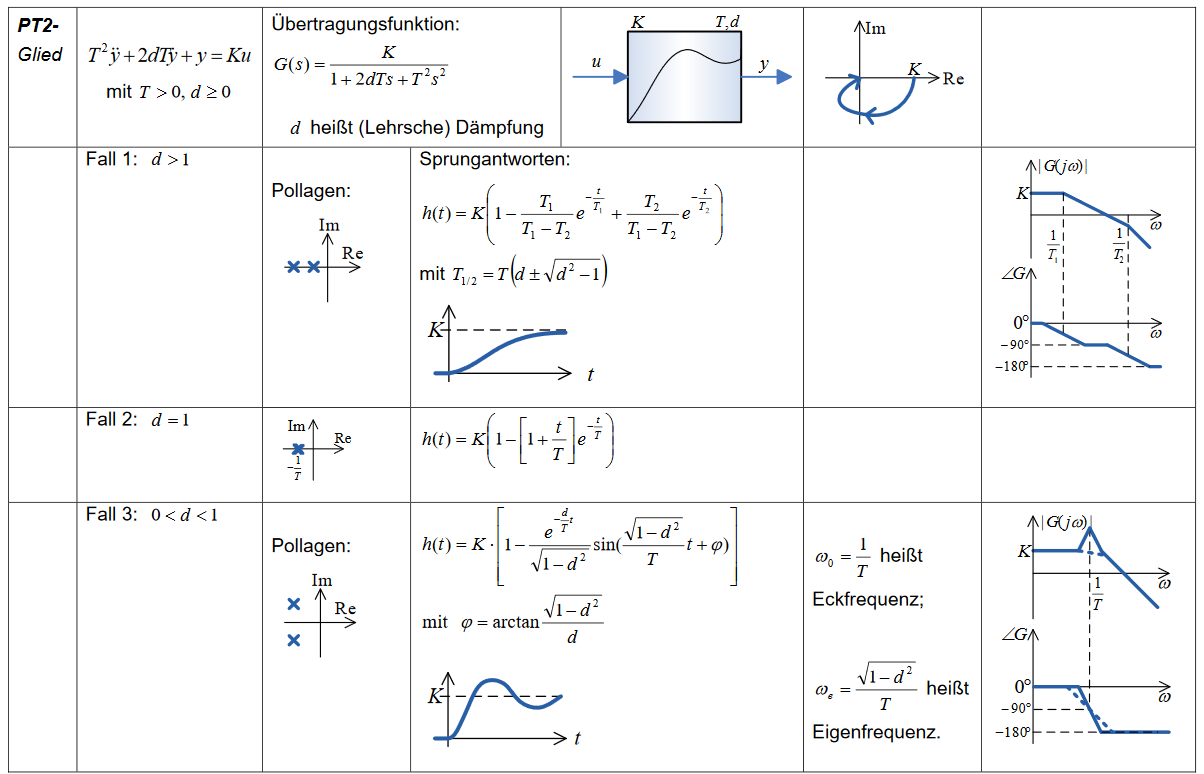
\includegraphics[width=1\columnwidth]{imgs/bb2_2c.png}
\end{figure}
\begin{figure}[H]
	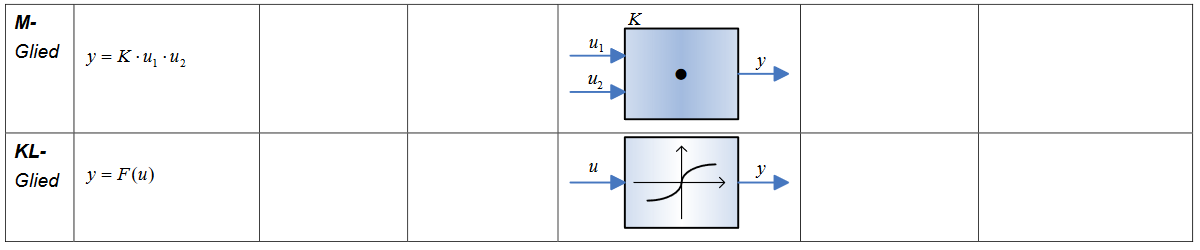
\includegraphics[width=1\columnwidth]{imgs/bb2_2d.png}
\end{figure}

Die Übertragungsglieder Summationsglied, Proportionalglied, Integrierglied, Differenzierglied und Totzeitglied sind linear.

\subsubsection{Sprungfunktion, Impulsfunktion}
\renewcommand{\arraystretch}{2}
$$
\begin{array}{ll}
	\text{Sprungfunktion} &	\sigma(t) = \begin{cases}
	0 & \text{für } t < 0 \\
	1 & \text{für } t ≥ 0
	\end{cases} \\
	\text{Impulsfunktion} & \delta(t) = \frac{d \sigma(t)}{dt} \\
	\text{Es gilt:} & \int_{-∞}^{∞} \delta(t) dt = 1 \\
	& \int_{-∞}^t \delta(t) dt = \sigma(t)
\end{array}
$$
\renewcommand{\arraystretch}{1.5}

\subsection{Lineare zeitinvariante Modelle (LZI-Modelle)}
\subsubsection*{Eigenschaften}
\begin{itemize}
	\item \textbf{Linearität:} Für $y(t) = \varphi(u(t))$ gilt:
	\begin{itemize}
		\item $\varphi(c_1 u_1(t) + c_2 u_2(t)) = c_1 \varphi(u_1(t)) + c_2 \varphi(u_2(t))$
	\end{itemize}
	\item \textbf{Zeitinvarianz:}
	\begin{itemize}
		\item $y(t) = \varphi(u(t))$ folgt $\varphi(u(t-T)) = y(t-T)$
	\end{itemize}
\end{itemize}

\subsubsection{Regelungsnormalform}
Das System $y^{(n)} + a_{n-1} y^{(n-1)} + \dots + a_1 \dot y + a_0 y = b_0 u$ \\
besitzt die Zustandsdarstellung
$$
	\dot x = \begin{bmatrix}
		0 & 1 & 0 & \dots & 0 \\
		0 & 0 & 1 & \ddots & \vdots \\
		\vdots & \vdots & \ddots & \ddots & 0 \\
		0 & 0 & \dots & 0 & 1 \\
		-a_0 & -a_1 & \dots & -a_{n-2} & -a_{n-1}
	\end{bmatrix} x + \vect{0 \\ \vdots \\ \vdots \\ 0 \\ b_0} u
$$
$$
	y = \vect{1 & 0 & \dots & 0} x
$$
Sie heißt Regelungsnormalform

\subsubsection{Regelungsnormalform mit Ableitungen von u}

Das System $y^{(n)} + a_{n-1} y^{(n-1)} + \dots + a_1 \dot y + a_0 y = b_{n-1} u^{n-1} + \dots + b_1 \dot u + b_0 u$ \\
besitzt die Zustandsdarstellung
$$
\dot x = \begin{bmatrix}
0 & 1 & 0 & \dots & 0 \\
0 & 0 & 1 & \ddots & \vdots \\
\vdots & \vdots & \ddots & \ddots & 0 \\
0 & 0 & \dots & 0 & 1 \\
-a_0 & -a_1 & \dots & -a_{n-2} & -a_{n-1}
\end{bmatrix} x + \vect{0 \\ \vdots \\ \vdots \\ 0 \\ 1} u
$$
$$
y = \vect{b_0 & b_1 & \dots & b_{n-1}} x
$$
Sie heißt Regelungsnormalform

\subsubsection{Beobachtungsnormalform}
Das System $y^{(n)} + a_{n-1} y^{(n-1)} + \dots + a_1 \dot y + a_0 y = b_{n-1} u^{n-1} + \dots + b_1 \dot u + b_0 u$ \\
besitzt die Zustandsdarstellung
$$
\dot x = \begin{bmatrix}
0 & 0 & \dots & 0 & -a_0 \\
1 & 0 & \ddots & 0 & -a_1 \\
0 & 1 & \ddots & 0 & -a_2\\
\vdots & \ddots & \ddots & 0 & \vdots \\
0 & \dots & 0 & 1 & -a_{n-1}
\end{bmatrix} x + \vect{b_0 \\ b_1 \\ b_2 \\ \vdots \\ b_{n-1}} u
$$
$$
y = \vect{0 & \dots & 0 & 1} x
$$
Sie heißt Beobachtungsnormalform

\subsection{Linearisierung im Arbeitspunkt}
\subsubsection{Ein Eingabeparameter} ~\\
Sei $y = F(u)$ eine Übertragungsfunktion. \\
Die linearisierte Funktion um den Arbeitspunkt $u_s$ ist berechnet als:
$$
	\Delta y = f(\Delta u, u_s) = \frac{\partial F(u)}{\partial u}\bigg|_{u = u_s} ⋅ \Delta u
$$
mit
$$
	\Delta y = y - y_s
$$
$$
	y_s = F(u_s)
$$
$$
	\Delta u = u - u_s
$$
Die um den Arbeitspunkt linearisierte Beziehung zwischen den absoluten Größen ist definiert als:
$$
	y_{lin} = f(u,u_s) = \Delta y + y_s \tab \text{(Ersetze $\Delta u$ durch $u - u_s$)}
$$

\subsubsection{Mehere Eingabeparameter} ~\\
Sei $y = F(u_1, \dots u_n)$ eine Übertragungsfunktion ($n \in \mathbb{N}$). \\
Die linearisierte Funktion um den Arbeitspunkt $(u_{1,s}, \dots, u_{n,s})$ wird wie folgt berechnet:
$$
\Delta y = f(\Delta u_1, \dots, \Delta u_n, u_{1,s}, \dots, u_{n,s}) = \frac{\partial F(u_1, \dots u_n)}{\partial u_1}\Bigg|_\textrm{AP} ⋅ \Delta u_1 + \dots + \frac{\partial F(u_1, \dots u_n)}{\partial u_n}\Bigg|_\textrm{AP} ⋅ \Delta u_n
$$
$$
	\textrm{AP} ≡ u_1 = u_{1,s}, \dots, u_n = u_{n,s}
$$
mit
$$
	\Delta y = y - y_s
$$
$$
	y_s = F(u_s)
$$
$$
	\Delta u_1 = u_1 - u_{1,s}, \dots, \Delta u_n = u_n - u_{n,s}
$$
Die um den Arbeitspunkt linearisierte Beziehung zwischen den absoluten Größen ist definiert als:
$$
y_{lin} = f(u_1, \dots, u_n, u_{1,s}, \dots, u_{n,s}) = \Delta y + y_s  \tab \text{(Ersetze $\Delta u_1$ durch $u_1 - u_{1,s}, \dots$)}
$$

\subsubsection{Regelungsnormalform}
Gegeben sei ein System in der Form $\dot x = Ax + ez + bu$, $y = c^T x$. \\
Die $n$ algebraischen Gleichungen seien definiert als: \\
$\begin{array}{l}
	f_1(x_1, \dots, x_n, z, u) = a_{11} x_1 + \dots + a_{1n} x_n + e_1 z + b_1 u \\
	\tab \vdots \\
	f_n(x_1, \dots, x_n, z, u) = a_{n1} x_1 + \dots + a_{nn} x_n + e_n z + b_n u
\end{array}$ \\
Die Ausgangsgröße sei definiert als:
$g(x_1, \dots, x_n) = y = c_1 x_1 + \dots + c_n x_n$ \\
Das linearisierte Modell wird wie folgt berechnet:
$$
	\Delta \dot x(t) = A_l \Delta x(t) + e_l \Delta z(t) + b_l \Delta u(t)
$$
$$
	\Delta y(t) = c_l^T \Delta x(t)
$$
$$
	A_l = \left. \begin{bmatrix}
		\frac{\partial f_1}{\partial x_1} & \dots & \frac{\partial f_1}{\partial x_n} \\
		\vdots & \ddots & \vdots \\
		\frac{\partial f_n}{\partial x_1} & \dots & \frac{\partial f_n}{\partial x_n} \\
	\end{bmatrix}\right |_\textrm{AP}
$$
$$
	e_l = \left.\vect{\frac{\partial f_1}{\partial z} \\ \vdots \\ \frac{\partial f_n}{\partial z}}\right |_\textrm{AP}
$$
$$
	b_l = \left.\vect{\frac{\partial f_1}{\partial u} \\ \vdots \\ \frac{\partial f_n}{\partial u}}\right |_\textrm{AP}
$$
$$
	c_l^T = \left.\vect{\frac{\partial g}{\partial x_1} & \dots & \frac{\partial g}{\partial x_n}}\right |_\textrm{AP}
$$

\section{Laplace-Transformation}
\begin{figure}[H]
	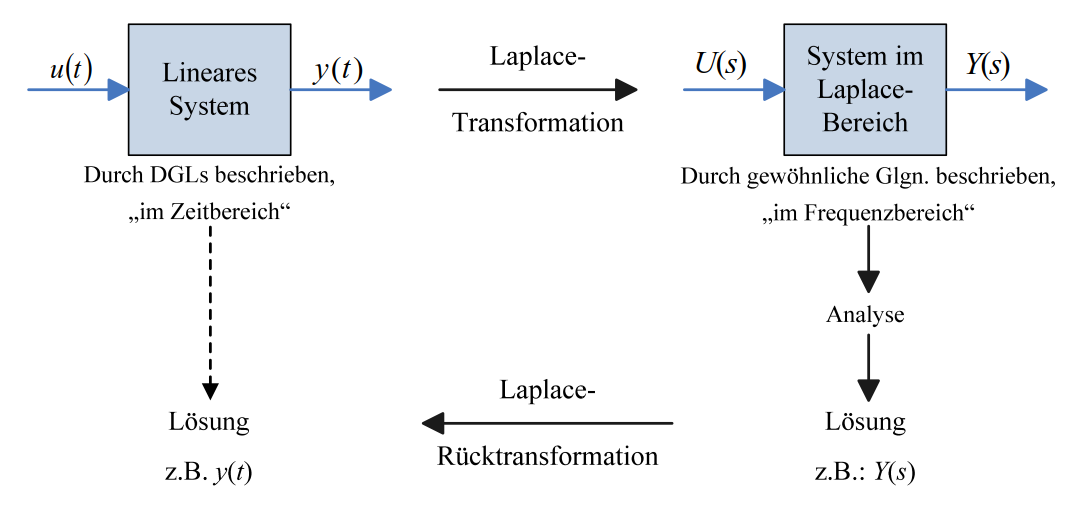
\includegraphics[width=0.8\columnwidth]{imgs/laplace.png}
\end{figure}

\subsection{Definition}
Sei $f(t)$ eine Zeitfunktion mit $f(t) = 0$ für $t < 0$. \\
Die Laplace-Transformierte dieser Zeitfunktion ist definiert als:
$$
	F(s) = \mathcal{L}\{f(t)\} = \int_0^{∞} f(t) e^{-st} dt
$$
wobei
$s = \delta + j \omega$ \\

Die Korrespondenz wird wie folgt dargestellt:
$$
	f(t) ~\laplace ~F(s)
$$

\subsection{Rücktransformation}
Sei $F(s)$ die Laplace-Transformierte zu $f(t)$. \\
Die Rücktransformation ist definiert als:
$$
	f(t) = \mathcal{L}^{-1}\{F(s)\} = \frac 1 {2\pi j} \int_{c - j ∞}^{c + j∞} F(s) e^{st} ds
$$
mit $c$ in der Konvergenzhalbebene.

\pagebreak
\begin{multicols}{2}
\subsection{Korrespondenztabelle}

\begin{tabularx}{\columnwidth}{|X|X|}
	\hline
	$f(t)$ & $F(s)$ \\
	\hline
	\hline
	$\delta(t)$ (Dirac-Impuls)& 1 \\
	\hline
	$\delta(t - t_0)$ & $e^{-t_0 s}$ \\
	\hline
	$\sigma(t)$ (Einheitssprung) & $\frac 1 s$ \\
	\hline
	$\sigma(t - t_0)$ & $\frac{e^{-t_0 s}}{s}$ \\
	\hline
	$t$ & $\frac{1}{s^2}$ \\
	\hline
	$\frac{t^n}{n!}, n \in \mathbb{N}_0$ & $\frac{1}{s^{n + 1}}$ \\
	\hline
	$e^{\alpha t}$ & $\frac{1}{s - \alpha}$ \\
	\hline
	$\frac 1 T e^{-\frac t T}$ & $\frac{1}{1 + Ts}$ \\
	\hline
	$te^{\alpha t}$ & $\frac{1}{(s - \alpha)^2}$ \\
	\hline
	$\frac{t}{T^2} e^{- \frac t T}$ & $\frac{1}{(1 + Ts)^2}$ \\
	\hline
\end{tabularx}
\begin{tabularx}{\columnwidth}{|X|X|}
	$\frac{t^n}{n!}e^{\alpha t}$ & $\frac{1}{(s - \alpha)^{n + 1}}$ \\
	\hline
	$1 - e^{\alpha t}$ & $\frac{-\alpha}{s(s - \alpha)}$ \\
	\hline
	$1 - e^{-\frac{t}{T}}$ & $\frac{1}{s(1 + Ts)}$ \\
	\hline
	$\sin \omega t$ & $\frac{\omega}{s^2 + \omega^2}$ \\
	\hline
	$\cos \omega t$ & $\frac{s}{s^2 + \omega^2}$ \\
	\hline
	$e^{-\delta t}\sin \omega t$ & $\frac{\omega}{(s + \delta)^2 + \omega^2}$ \\
	\hline
	$e^{-\delta t}\cos \omega t$ & $\frac{s + \delta}{(s + \delta)^2 + \omega^2}$ \\
	\hline
	$t \sin \omega t$ & $\frac{2 \omega s}{(s^2 + \omega^2)^2}$ \\
	\hline
	$t \cos \omega t$ & $\frac{s^2 - \omega^2}{(s^2 + \omega^2)^2}$ \\
	\hline	
\end{tabularx} \\
\\

wobei \\
$f(t) = 0$ für $t < 0$, \\
$T > 0, t_0 > 0, \omega > 0$ reell, \\
$\delta$ beliebig reell und \\
$\alpha$ beliebig komplex.
\end{multicols}

\subsection{Eigenschaften der Laplace-Transformation}
\begin{tabularx}{\columnwidth}{|X|X|X|}
	\hline
	Eigenschaft & Operation im Zeitbereich & Operation im Bildbereich \\
	\hline
	\hline
	Linearität & $c_1f_1(t) + c_2f_2(t)$ & $c_1 F_1(s) + c_2 F_2(s)$ \\
	\hline
	Differenziation & $\dot f(t)$ & $sF(s) - f(0)$ \\
	& $f^{(n)}(t)$ & $s^n F(s) - s^{n - 1} f(0) - \dots - f^{(n-1)}(0)$ \\
	\hline
	Integration & $\int_0^t f(\tau) ~d\tau$ & $\frac 1 s F(s)$ \\
	\hline
	Dämpfung & $f(t) ⋅ e^{\alpha t}$ & $F(s-\alpha)$ \\
	\hline
	Faltung & $f_1(t) * f_2(t)$ & $F_1(s) ⋅ F_2(s)$ \\
	\hline
	Zeitverschiebung & $f(t - t_0), t_0 > 0$ & $e^{-t_0 s}F(s)$ \\
	\hline
	Diffenrentiation der Bildfunktion & $(-1)^n t^n f(t)$ & $F^{(n)}(s), n \in \mathbb{N}$ \\
	\hline
	Skalierung der Zeitachse & $f(\alpha t), \alpha > 0$ & $\frac 1 \alpha F(\frac s \alpha)$ \\
	\hline
	Anfangswertsatz & \multicolumn{2}{X|}{$\lim_{t → +0} f(t) = \lim_{s → ∞} s F(s)$, sofern $\lim_{t → +0} f(t)$ existiert} \\
	\hline
	Endwertsatz & \multicolumn{2}{X|}{$\lim_{t → ∞} f(t) = \lim_{s → 0} sF(s)$, sofern $\lim_{t → ∞} f(t)$ existiert} \\
	\hline
\end{tabularx}

\subsection{Lösung linearer zeitinvarianter Differentialgleichungen mittels Laplace-Transformation}
Sei $a_ny^{(n)} + \dots + a_1 \dot y + a_0 y = b_m u^{(m)} + \dots + b_1 \dot u + b u$ mit $m ≤ n$ und $a_n ≠ 0$ die systembeschreibende Differentialgleichung.
Die Lösung dieser DGL erfolgt durch die folgenden 5 Schritte:
\begin{enumerate}
	\item Transformation der DGL in den Bildbereich mittels Laplace-Transformation
	\item Auflösen nach $Y(s)$. Sind alle Anfangswerte gleich null, resultiert: \\
	$Y(s) = \frac{b_ms^m + \dots + b_1s + b_0}{a_ns^n + \dots + a_1s + a_0} U(s) ≡ Y(s) = G(s) ⋅ U(s)$
	\item Einsetzen von $U(s) ~\Laplace ~u(t)$ in $Y(s) = G(s) ⋅ U(s)$
	\item Durchführung einer Partialbruchzerlegung von $Y(s)$
	\item Rücktransformation in den Zeitbereich $y(t) ~\laplace ~Y(s)$
\end{enumerate}

\subsubsection{Darstellungsformen von G(s)}
\label{darstell_gs}
$G(s)$ kann in folgenden Formen dargestellt werden: \\
\begin{tabular}{lll}
	Polynomform: & $G(s) = \frac{b_ms^m + \dots + b_1s + b_0}{a_ns^n + \dots + a_1s + a_0}$ \\
	Linearfaktorform: & $G(s) = Q \frac{(s - q_1) ⋅ \dots ⋅ (s - q_m)}{(s - p_1)⋅ \dots ⋅ (s - p_n)}$ & mit $Q = \frac{b_m}{a_n}$ \\
	Zeitkonstantenform: & $G(s) = K \frac{(1 + \bar{T}_1 s) ⋅ \dots ⋅ (1 + \bar{T}_m s)}{(1 + T_1s) ⋅ \dots ⋅ (1 + T_n s)}$ & mit $\bar{T}_i = - \frac 1 {q_i}$, $T_i = -\frac 1 {p_i}$, $K = \frac{b_0}{a_0}$ \\
	Partialbruchform: & $G(s) = r_0 + \frac{r_1}{s - p_1} + \dots + \frac{r_n}{s - p_n}$
\end{tabular}

\subsubsection{Komplexe Übertragungsfunktion}
Sei $Y(s) = G(s)U(s)$ eine systembeschreibende Differentialgleichung im Bildbereich. \\
$G(s) = \frac{Y(s)}{U(s)}$ heißt komplexe Übertragungsfunktion. \\
Komplexe Übertragungsfunktionen der in Sektion \ref{darstell_gs} genannten Darstellungsformen heißen rationale Übertragungsfunktionen. Die zugehörigen Übertragungsglieder heißen rationale Übertragungsglieder, kurz R-Glieder.

\subsection{Sprungantworten des PT2-Gliedes}
Die Pole von der komplexen Übertragungsfunktion $G(s)$ eines PT2-Gliedes werden wie folgt berechnet:
$$
	p_{1/2} = \frac 1 T (-d \pm \sqrt{d^2 - 1})
$$
Es folgt: \\
\begin{tabular}{llll}
	Fall 1: & $d > 1$, & $p_{1/2} \in \mathbb{R}^-$, & aperiodischer Fall \\
	Fall 2: & $d = 1$, & $p_1 = p_2, p_{1/2} \in \mathbb{R}^-$, & aperiodischer Grenzfall \\
	Fall 3: & $0 < d < 1$, & $p_{1/2} \in \mathbb{C}, \Re(p_{1/2}) < 0$, & unterkritisch/periodisch gedämpfter Fall \\
	Fall 4: & $d = 0$, & $p_{1/2} \in \mathbb{C} \backslash \mathbb{R}$, & ungedämpfter Fall
\end{tabular}

\subsection{Lösung der Zustandsgleichung mittels Laplace-Transformation}
Sei ein LZI-System gegeben mit $\dot x = Ax + bu$ und $y = c^T x$. \\
Die Zustandsgleichungen im Bildbereich sind:
$$
	X(s) = (sI-A)^{-1} b U(s) + (sI-A)^{-1} x(0) ~\Laplace ~x(t)
$$
$$
	Y(s) = c^T(sI-A)^{-1} b U(s) + c^T (sI - A)^{-1} x(0) ~\Laplace ~y(t)
$$
Die komplexe Übertragungsfunktion $G(s)$ ist:
$$
	G(s) = c^T(sI - A)^{-1} b = \frac{c^T(\textrm{Adjunkte}(sI-A))b}{\det(sI-A)} = \frac{Z(s)}{N(s)}
$$

\subsubsection{Polstellen}
Jeder Pol von $G(s)$ ist Eigenwert von $A$. Ein Eigenwert von $A$ ist genau dann Pol von $G(s)$, wenn er sich nicht herauskürzt, d.h. nicht gleichzeitig Nullstelle von $Z(s)$ ist.

\subsubsection{Zustandsgleichung mit Störgröße}
Seien die Zustandsgleichungen des LZI-Systems gegeben durch $\dot x = Ax + ez + bu$ und $y = c^T x$. \\
Die Zustandsgleichung im Bildbereich ist:
$$
	Y(s) = G(s) U(s) + G_z(s) Z(s)
$$
und die Störübertragungsfunktion ist
$$
	G_z(s) = c^T(sI-A)^{-1}e
$$

\subsection{Lösung der Zustandsgleichungen im Zeitbereich}
Sei ein LZI-System gegeben mit $\dot x = Ax + bu$ und $y = c^T x$. \\
Die Lösungen dieser Gleichungen sind:
$$
	x(t) = \int_0^t e^{A(t-\tau)} b u(\tau) ~d\tau + e^{At} x(0)
$$
$$
	y(t) = \int_0^t c^T e^{A(t-\tau)} bu(\tau) ~d\tau + c^T e^{At} x(0)
$$
wobei
$$
	e^{At} = I + A\frac{t}{1!} + A^2 \frac{t^2}{2!} + \dots
$$

\subsubsection{Transitionsmatrix}
Die Matrix $e^{At}$ heißt Überführungs- bzw. Transitionsmatrix.
Sie hat folgende Eigenschaften.
$$
	e^{At} ⋅ e^{A\tau} = e^{A(t + \tau)}
$$
$$
	e^{-At} ⋅ e^{At} = e^0 = I
$$
$$	
	\frac{d e^{At}}{dt} = Ae^{At} = e^{At} A
$$

\section{Analyse dynamischer Systeme}




\pagebreak
\section{Mathematische Grundlagen}
\subsection{Komplexe Zahlen}
\subsubsection{Definition}
Eine komplexe Zahl $z \in \mathbb{C}$ ist definiert als:
$$
	z = x + jy
$$
wobei $x, y \in \mathbb{R}$ und
$j = \sqrt{-1}$ ist die imaginäre Einheit. \\

Der Real- und Imaginärteil ist definiert als:
$$
	\Re(z) = x, \tab 	\Im(z) = y
$$

\subsubsection{Konjugiert komplexe Zahl}
Sei $z \in \mathbb{C}$. \\
Die zu $z$ konjugiert komplexe Zahl $z^*$ ist:
$$
	z^* = x - jy
$$

\subsubsection{Betrag einer komplexen Zahl}
Sei $z \in \mathbb{C}$. \\
Der Betrag von $z$ ist:
$$
	|z| = \sqrt{x^2 + y^2}
$$

\subsubsection{Euler-Formel}
$$
e^{j\varphi} = \cos \varphi + j \sin \varphi
$$

\subsubsection{Polarkoordinaten}
Sei $z \in \mathbb{C}$. \\
$z$ angegeben in Polarkoordinaten ist definiert als:
$$
	z = |z|(\cos \varphi + j \sin \varphi) = |z|e^{j\varphi}
$$
wobei \\
$\varphi = \arg(z) = \begin{cases}
	\arctan(\frac y x) & $für $x > 0 \\
	\pi + \arctan(\frac y x) & $für $x < 0
\end{cases}
$

\subsubsection{Addition, Multiplikation}
Sei $z_1, z_2 \in \mathbb{C}$. \\
Es folgt:
$$
	z_1 + z_2 = (x_1 + x_2) + j(y_1 + y_2)
$$
$$
	z_1 ⋅ z_2 = (x_1x_2 - y_1y_2) + j(x_1y_2 + y_1x_2)
$$
$$
	z_1 ⋅ z_2 = |z_1| ⋅ |z_2| ⋅ e^{j(\varphi_1 + \varphi_2)}
$$



%TODO Partialbruchzerlegung
%TODO Matrizenrechnung

\section{Elektrotechnische Grundlagen}
\subsection{Widerstand}
\textbf{Schaltzeichen:} \\
\begin{figure}[H]
	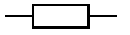
\includegraphics[width=0.15\columnwidth]{imgs/widerstand.pdf}
\end{figure}
\textbf{Formel:}
$$
	U = R ⋅ I
$$

\subsection{Kondensator}
\textbf{Schaltzeichen:} \\
\begin{figure}[H]
	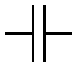
\includegraphics[width=0.1\columnwidth]{imgs/kondensator.pdf}
\end{figure}
\textbf{Formel:}
$$
	U = \frac 1 C \int I \textrm{ dt} \iff \dot U = \frac I C
$$

\subsection{Spule}
\textbf{Schaltzeichen:} \\
\begin{figure}[H]
	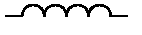
\includegraphics[width=0.1\columnwidth]{imgs/spule.pdf} bzw. 
	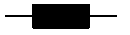
\includegraphics[width=0.1\columnwidth]{imgs/spule_alt.pdf}	
\end{figure}
\textbf{Formel:}
$$
	U = L ⋅ \dot I
$$

\subsection{Kirchoff'sches Spannungsgesetz}
In einem geschlossenen Stromkreis (Masche) ist die Summe aller Spannungen gleich null \\

\textbf{Beispiel:}
\begin{figure}[H]
	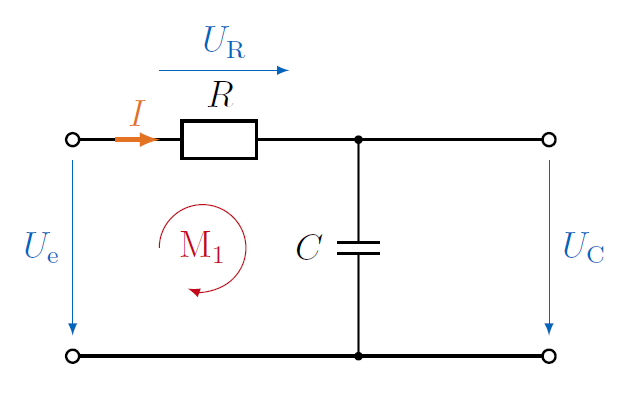
\includegraphics[width=0.5\columnwidth]{imgs/kvl.png}
\end{figure}
Für Masche $M_1$ gilt:
$$
U_R + U_C - U_e = 0
$$

\subsection{Kirchoff'sches Stromgesetz}
In jedem Knotenpunkt ist die Summe aller Ströme gleich null.

\textbf{Beispiel:}
\begin{figure}[H]
	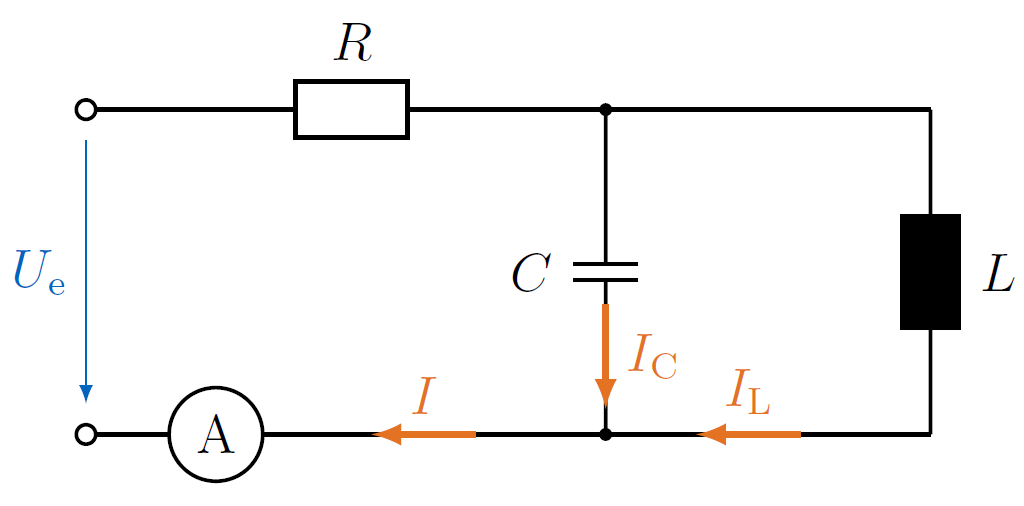
\includegraphics[width=0.5\columnwidth]{imgs/kcl.png}
\end{figure}
$$
	I_C + I_L - I = 0
$$

\section{Physikalische Grundlagen}
\subsection{Kräfte}
\textbf{Kräftegleichgewicht:} \\
Die Summe aller Kräfte, die an einem Körper angreifen, addieren sich zu null.
$$
	\sum F_i = 0
$$

\textbf{Newtonsche Gesetze}
\begin{enumerate}
	\item Wirkt auf einen Körper keine Kraft oder befindet er sich im Kräftegleichgewicht, so bleibt er in Ruhe oder er bewegt sich mit konstanter Geschwindigkeit geradlinig weiter.
	\item $F = m ⋅ a$ \tab[2] ($m$: Masse des Körpers, $a$: Beschleunigung, die der Körper erfährt)
	\item $F_1 = -F_2$ \tab[2] (Kraft gleich Gegenkraft)
\end{enumerate}

\textbf{Masse-Feder-Dämpfer System}
\begin{figure}[H]
	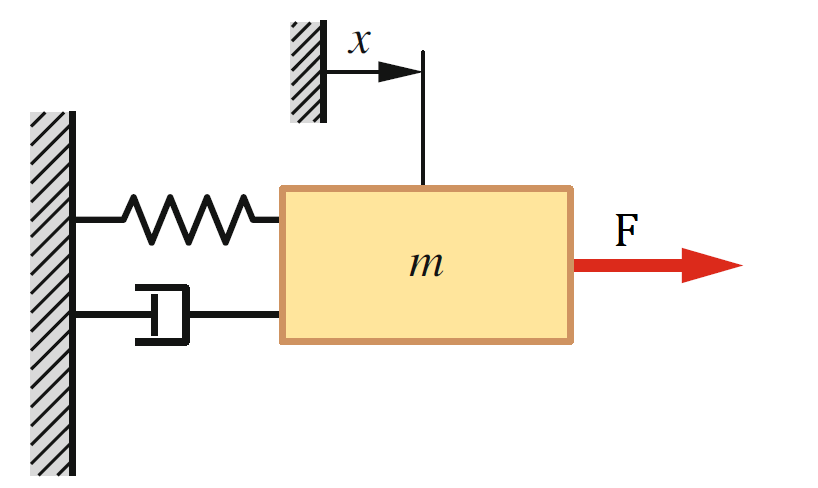
\includegraphics[width=0.5\columnwidth]{imgs/mass-spring-damper.png}
\end{figure}
$m$: Masse des Körpers, $d$: Dämpferkonstante, $k$: Federkonstante, $F$: Stellkraft
$$
	F = m ⋅ \ddot x + d \dot x + k x
$$


\subsection{Drehmomente}
\textbf{Momentengleichgewicht:} \\
Die Summe aller Momente um jeden (einen) beliebigen Punkt eines Körpers addieren sich zu null.
$$
	\sum M_i = 0
$$

\textbf{Berechnung in Abhängigheit von F:} \\
$r$: Abstand der Wirkungslinie der Kraft von der Drehachse, $F$: wirkende Kraft
$$
	M = r \times F
$$

\subsection{Drehimpuls:}
$J$: Trägheitsmoment, $\omega$: Winkelgeschwindigkeit
$$
	L = J ⋅ \omega
$$


\section{Tipps}
\subsection{Zeichnen eines Blockschaltbildes}
\begin{itemize}
	\item Verzweigungen von Signalen werden durch einen schwarzen Punkt markiert, um die Verwechslungsgefahr mit Kreuzungen ohne Kontakt zu vermeiden.
	\item Signale werden immer explizit mit Summationsgliedern aufaddiert.
	\item Proportionalitätsfaktoren von 1 können weggelassen werden.
	\item Das Vorzeichen beim Summationsglied steht immer rechts vom Pfeil. Die Pluszeichen müssen nicht explizit angegeben werden.
	\item Das Vorzeichen einer Rückführung steht am Soll-/Istwert-Vergleich
\end{itemize}
\textbf{Allgemeine Vorgehensweise:}
\begin{enumerate}
	\item Differentialgleichung nach höchster Ableitung auflösen
	\item $n$ I-Glieder mit zugehörigen Anfangswerten nebeneinander zeichnen, verbinden und beschriften
	\item Summationsglieder für die höchste Ableitung bilden
	\item Jeden Term der rechten Seite aus bestehenden Signalen bilden
\end{enumerate}

%TODO Beispiel




\pagebreak
\section*{Anmerkungen}
Dies ist eine Zusammenfassung der Vorlesung Regelungstechnik an der Technischen Universität München.
Gehalten wurde diese Vorlesung durch Lohmann B. im Sommersemester 2019.
Ersteller dieser Zusammenfassung ist Gaida B.
Alle Angaben sind ohne Gewähr.


\section*{Literaturverzeichnis}
Werner Skolaut. \textit{Maschinenbau. Ein Lehrbuch für das ganze Bachelor-Studium}. Springer Vieweg. Heidelberg, 2018, S. 1271 - 1387





\end{document}

%TODO check for todos








